\documentclass[11pt]{article}
\usepackage[utf8]{inputenc}
\usepackage[italian]{babel}
\usepackage{amssymb}
\usepackage{verbatim}
\usepackage{amsfonts}
\usepackage{amsmath}
\usepackage{multirow}
\usepackage{amsthm}
\usepackage{xcolor}
\usepackage{graphicx}
\usepackage{tikz}
\usepackage{float}
\usepackage[shortlabels]{enumitem}
\graphicspath{ {./images/} }
\usetikzlibrary{arrows}

\tikzset{
  treenode/.style = {align=center, inner sep=0pt, text centered,
    font=\sffamily},
  arn_n/.style = {treenode, circle, blue, font=\sffamily\bfseries, draw=blue,
    fill=white, text width=1.5em},% arbre rouge noir, noeud noir
  arn_r/.style = {treenode, circle, red, draw=red, 
    text width=1.5em, very thick},% arbre rouge noir, noeud rouge
}


\begin{comment}
\newcolumntype{+}{>{\global\let\currentrowstyle\relax}}
\newcolumntype{-}{>{\currentrowstyle}}
\newcommand{\rowstyle}[1]{\gdef\currentrowstyle{#1}#1\ignorespaces}
\end{comment}

%%%%%%%% cella testo spezzato %%%%%%%%%%
\newcommand{\splitcell}[2][c]{%
  \begin{tabular}[c]{@{}c@{}}\strut#2\strut\end{tabular}%
}

\title{Linguaggi e Computabilità}
\author{Daniele De Micheli}
\date{2019}

\renewcommand*\contentsname{\textit{Indice}}


%presettaggio per teoremi e assiomi/definizioni%

\newtheorem*{problemaDecisione}{Problema di Decisione}
\newtheorem*{problemaMembership}{Problema di Membership}
\newtheorem{relazioneNorm}{Prima relazione}
\newtheorem{relazioneStar}{Seconda relazione}
\newtheorem{alberoSintattico}{Albero Sintattico}
\newtheorem{eqEnunciati}{Equivalenza degli enunciati}
\newtheorem{ambiguitaSinistra}{Teorema}



%fine%

\begin{document}

\maketitle
\tableofcontents
\part{Prima Parte}
\section{Alfabeti e Linguaggi}
Si definisce \textbf{alfabeto} un insieme finito e non vuoto di simboli. Ad esempio, l'alfabeto $\{A,B,C,...,Z\}$ potremmo definirlo come l'insieme delle lettere maiuscole dell'alfabeto italiano. Altri esempi intuitivi sono l'inseme delle cifre che compongono i numeri arabi $\{1,2,3,...9,0\}$ o l'insieme $\{0,1\}$ che rappresenta i numeri binari. Un alfabeto si indica con una lettera maiuscola
greca:
\begin{itemize}
	\item $A=\{A,B,C,...,Z\}$;
	\item $\Gamma = \{0,1\}$;
\end{itemize}
Si definisce invece una \textbf{stringa} un insieme vuoto, finito o infinito di simboli presi da un dato alfabeto. Una stringa vuota si indica con $\epsilon o \lambda$.
\subsection{Stringhe}
Una stringa, come abbiamo già visto, si rappresenta con una lettera greca
maiuscola. Nel caso volessimo indicare invece la lunghezza di una stringa
bisogna utilizzare la seguente notazione: $$|\Gamma | = x$$ dove $\Gamma$ rappresenta la stringa e x la sua lunghezza.
\\ \\
Le stringhe possono inoltre essere "manipolate", o meglio esse si possono \textit{concatenare} per ottenere una nuova stringa. Tale operazione si può indicare così: $\Gamma \circ A$ e si legge "$\Gamma \medspace concatenata \medspace ad \medspace A$". La concatenazione \textbf{non} è un'operazione commutativa. Infatti $$\Gamma \circ A \neq A \circ \Gamma$$

Se prendiamo ad esempio $A = \{010\}$ e $\Gamma = \{11\}$, allora $A \circ \Gamma = \{01011\}$ mentre $\Gamma \circ A = \{11010\}$ che non sono assolutamente uguali come si può ben vedere.

\subsection{Alfabeti}
Gli alfabeti, come abbiamo già visto, sono insieme finiti di simboli. Su tali
insiemi  è possibile definire delle operazioni che generano delle stringhe a
partire dall'alfabeto stesso.

\paragraph{Potenza di un alfabeto}: dato un alfabeto $E$, si definisce \textit{potenza di E} la stringa di lunghezza k contenente tutti gli elementi dell'alfabeto $E$.
$$dato \medspace E, k \geq 0 \in \mathbb{Z}, \Rightarrow E^k = E\times E\times E\times E \times ... \times E, k \medspace volte$$

Se $|E| = q$, allora $|E^k| = q^k$. Ad esempio, prendiamo l'alfabeto $E=\{0,1\}$. Allora:
\begin{itemize}
	\item $E^1 = \{0,1\}$
	\item $E^2 = \{00,01,10,11\}$
	\item $E^3 = \{000,001,010,011,100,101,110,111\}$
\end{itemize}
Come si può intuire dall'esempio qui sopra, il risultato della potenza di un alfabeto non è altro che l'insieme delle \textit{combinazioni} di numero k degli elementi dell'alfabeto.

\paragraph{Chiusura di Kleene}: la chiusura di Kleene è un'operazione che riguarda
le potenze di un alfabeto. Infatti tale operazione non è altro che l'unione di
tutte le potenze di un alfabeto fino a k. Formalmente: $$E^{\star} = \cup E^k = E^0 \cup E^1 \cup E^2 ... \cup E^k, \medspace t.c. \medspace k\geq 0$$

Un'operazione derivata da quest'ultima è la chiusura di Kleene ma senza l'elemento 0: $$E^{+}=E^{\star}\setminus E^0$$

\subsection{Linguaggio} Possiamo definire un \textit{linguaggio} $L \medspace su \medspace E$ un sottoinsieme di $E^{\star}$ tale che $L \subseteq E^{\star}$. Per esempio, preso $E = \{a,b,c\}$, un linguaggio L potrebbe essere $L_{1}=\{aa,cbc\}$. Un linguaggio può essere finito (vedi $L_ {1}$), oppure infiniti (es. $L_{2} = \{ w \in E^{\star} \thickspace | \thickspace w \medspace contiene \medspace lo \medspace stesso \medspace numero \medspace di \medspace a \medspace e \medspace c\}$).
\\ \\
Preso un linguaggio $L \subseteq E^{\star}$, possiamo affermare che:
\begin{itemize}
\item[1.] $ \emptyset \subseteq L$;
\item[2.] $ \varepsilon \subseteq L $;
\item[3.] $ E^{\star} \subseteq L$;
\end{itemize}
sono tutti linguaggi. La principale caratteristica di un linguaggio è che esso deve essere riconosciuto e interpretato da una macchina (o automa) ed essa deve anche essere in grado di generarlo tramite una \textbf{\textit{grammatica}}.
\begin{problemaDecisione}
Il problema di decisione si presenta nel momento in cui, dato un quesito, le possibili risposte sono sempre e sole "sì" o "no".
\end{problemaDecisione}
\begin{problemaMembership}
Il problema di Memebership è legato al concetto di stringa (come input), di linguaggio e di appartenenza ad un determinato linguaggio. Data una stringa w in input, una determinata macchina deve essere in grado di dire se essa appartiene ad un linguaggio oppure no.
\end{problemaMembership}

\textbf{\textit{DEFINIZIONI}}
Una \textbf{forma sentenziale} è una stringa di simboli terminali e non terminali: $\gamma \in (V \cup T)^{\star}$

\paragraph{Concatenazione di linguaggi}: Dati due linguaggi $L_1, L_2 \subseteq E^{\star}$ allora $$L_1 \circ L_2 = \{ w | w = w_1 \circ w_2, w_1 \in L_1, w_2 \in L_2\} $$
\subsection{Grammatiche}
La descrizione grammaticale di un linguaggio consiste di quattro componenti:
\begin{enumerate}
	\item Un insieme finito di simboli che formano le stringhe del linguaggio. Questi sono chiamati \textit{terminali} o \textit{simboli terminali}.
	\item Un insieme finito di \textit{variabili}, dette anche \textit{non terminali} o \textit{categorie sintattiche}. Ognuna di esse rappresenta un linguaggio.
	\item Una variabile, chiamata \textit{simbolo iniziale}, che rappresenta il liunguaggio da definire.
	\item Un insieme finito di \textit{produzioni}, o \textit{regole}, che rappresentano la definizione ricorsiva di un linguaggio. Ogni produzione consiste di tre parti:
	\begin{itemize}
		\item Una variabile che viene definita dalla produzione ed è spesso detta la \textbf{testa} della produzione.
		\item Il simbolo di produzione $\rightarrow$.
		\item Una stringa di zero o più terminali e variabili. detta il \textbf{corpo} della produzione, il quale rappresenta un modo di formare le stringhe nel linguaggo della variabile di testa. 
	\end{itemize}
\end{enumerate}
\subsubsection{Grammatica libere dal contesto}
Una grammatica context-free (CFG, Context Free Grammatic) è una grammatica che non prevede l'incrocio dei simboli terminali per cui è necessario utilizzare delle regole differenti. Possiamo rappresentare una CFG per mezzo dei quattro componenti descritti sopra, ossia $G=(V,T,P,S)$, dove $V$ è l'insieme delle variabili, $T$ i terminali, $P$ l'insieme delle produzioni ed $S$ il simbolo iniziale.
\\ \\
\paragraph{Stringhe palindrome}: le stringhe palindrome sono un esempio semplice di linguaggio che utilizza una grammatica context-free.
Abbiamo il l'alfabeto $E = \{0,1\}$ e il linguaggio costruito su esso $L_{pal} \subseteq E^{\star}$. Da questo alfabeto e con questo linguaggio possiamo costruire una stringa w palondroma come $$w = \{0110\}$$
Essa può essere definita per induzione come segue:
\begin{enumerate}
\item Passo base: $\varepsilon , 0, 1 \in L_{pal}$
\item Passo induttivo: se $w \in L_{pal}$, allora $0w0, 1w1, \varepsilon \in L_{pal}$
\end{enumerate}
Un esempio di regole del linguaggio possono essere:
\begin{equation}
\begin{split}
\color{red}S \color{black} \rightarrow \color{blue}\varepsilon\color{black}\\&\\
\color{red}S \color{black} \rightarrow \color{blue}0 \color{black}\\&\\
\color{red}S \color{black} \rightarrow \color{blue}1 \color{black}\\&\\ 
\color{red}S \color{black} \rightarrow \color{blue}0S0 \color{black}\\&\\
\color{red}S \color{black} \rightarrow \color{blue}1S1\color{black}
\end{split}
\end{equation}
in cui la \color{red} \textbf{testa} \color{black} può essere sostituita dal \color{blue} \textbf{corpo}\color{black}.
\\ \\
Queste regole possono essere applicate tramite le due \emph{relazioni}:
\begin{enumerate}
\item $\Rightarrow$
\item $\Rightarrow^{\star}$
\end{enumerate}
La prima (1) possiamo definirla come segue:
\begin{relazioneNorm}
Sia $G=(V, T,P,S)$ una CFG e sia $\alpha A \beta$ tale che $\alpha,\beta \in (V\cup T)^{\star}$ e $A \in V$. Sia $A \rightarrow \gamma \in P$. Allora $\alpha A\beta \Rightarrow \alpha \gamma \beta$.
\end{relazioneNorm}
\begin{relazioneStar}
Si ha che $\alpha \Rightarrow^{\star} \beta$, con $\alpha, \beta \in (V \cup T)^{\star}$, se e solo se $\exists \medspace \gamma_{1}, \gamma_{2}, ... ,\gamma_{n} \in (V\cup T)^{\star}$ tale che $\alpha \Rightarrow \gamma_{1} \Rightarrow \gamma_{2} \Rightarrow \gamma_{3} \Rightarrow ... \Rightarrow \gamma_{n} \Rightarrow \beta$ con $n \geq 1$.
Se n = 1, allora $\alpha = \beta$ e vale $\alpha \Rightarrow^{\star} \beta$ cioè $\alpha \Rightarrow^{\star} \gamma$.
\end{relazioneStar}
Le produzioni di una CFG si applicano per dedurre se una stringa può appartenere al linguaggio oppure no. Per fare questo si possono utilizzare due metodi differenti. Prese le seguenti regole (Regole 1.4.1)
\begin{enumerate}
	\item $E \rightarrow I$
	\item $E \rightarrow E+E$
	\item $E \rightarrow E*E$
	\item $E \rightarrow (E)$
	\item $I \rightarrow a$
	\item $I \rightarrow b$
	\item $I \rightarrow Ia$
	\item $I \rightarrow Ib$
	\item $I \rightarrow I0$
	\item $I \rightarrow I1$
\end{enumerate}
e questa stringa $w = a*(a+b00)$. Possiamo a questo punto intraprendere due strade per affermare se la stringa $w$ appartiene al linguaggio, quella della \textit{inferenza ricorsiva} o quella della \textit{derivazione}.
La prima funzina così: creo una tabella (\ref{tab:InfRic}) in cui in ogni passaggio applico una regola specificando per quale linguaggio e quali altre precedenti stringhe già ottenute sto riutilizzando.
\begin{table}[H]
\caption{Inferenza Ricorsiva}
\center
\label{tab:InfRic}
\begin{tabular}{c|c|c|c|c}

\textbf{n} & \textbf{\splitcell{Stringa\\ricavata}} & \textbf{Linguaggio} & \textbf{\splitcell{Produzione\\impiegata}} & \textbf{\splitcell{Stringhe\\impiegate}} \\
\hline
(i) & a & I & 5 & -- \\
(ii) & b & I & 6 & -- \\
(iii) & b0 & I & 9 & (ii) \\
(iv) & b00 & I & 9 & (iii) \\
(v) & a & E & 1 & (i) \\
(vi) & b00 & E & 1 & (iv) \\
(vii) & a + b00 & E & 2 & (v),(vi) \\
(viii) & (a + b00) & E & 4 & (vii) \\
(ix) & a * (a + b00) & E & 3 & (v),(viii) \\
\end{tabular}
\end{table}
L'altro metodo, quello per \textit{derivazione} prevede invece l'uso delle \textit{relazioni} viste nel paragrafo (1.4.1). La stessa stringa è quindi ottenuta nel seguente modo:

\begin{flalign*}
& E \Rightarrow_{lm} E * E \Rightarrow_{lm} I * E \Rightarrow_{lm} a * E \Rightarrow_{lm} &&\\\nonumber
& \Rightarrow_{lm}a * (E) \Rightarrow_{lm} a * (E+E) \Rightarrow_{lm} a * (I + E) \Rightarrow_{lm} a*(a+E)\Rightarrow_{lm} &&\\\nonumber
& \Rightarrow_{lm}a* (a+I)\Rightarrow_{lm}a*(a+I0)\Rightarrow_{lm}a*(a+I00)\Rightarrow_{lm}\textbf{$a*(a+b00)$}&&\\\nonumber
\end{flalign*}

Per ricavare la stringa abbiamo utilizzato una \textit{derivazione sinistra}, ma avremmo potuto eseguire la \textit{derivazione destra} e il risultato sarebbe stato il medesimo. Infatti, \textit{qualunque derivazione ha una derivazione a sinistra e una a destra \textbf{equivalenti}}. Eseguire una derivazione destra significa infatti applicare la derivazione prima all'elemento più a destra, fino ad arrivare a quello più a sinistra una volta risolta la derivazione.
\\ \\
\subsubsection{Grammatiche regolari}
Il linguaggio di esempio (di tipo 2): $L = \{w \in \{a,b,c\}^{\star} | w = a^nb^nc^n, n\geq 1\}$
è generato dalla seguente grammatica (NON context-free): $$ G=(\{S,X,B,C\}, \{a,b,c\}, P, S)$$
e dove le regole di produzione sono:
\begin{enumerate}
	\item $S \rightarrow aSBC$
	\item $S \rightarrow aBC$
	\item $CB \rightarrow XB$
	\item $XB \rightarrow XC$
	\item $XC \rightarrow BC$
	\item $aB \rightarrow ab$
	\item $bB \rightarrow bb$
	\item $bC \rightarrow bc$
	\item $cC \rightarrow cc$
\end{enumerate}
Le grammatiche 3,4,5 possono essere "collassate" in $CB \rightarrow BC$
Si può dimostrare , usando il Pumping Lemma per i CFL, che non è context-free.
\\ \\
Esempio di Derivazione:
\\ \\
Deriviamo la stringa abc (corrispondente a n = 1), indicando anche ad ogni passo la regola usata.
$$ S (2)\rightarrow aBC (6)\rightarrow abC (8)\rightarrow abc$$
Deriviamo la stringa aabbcc (corrispondente a n = 1), indicando anche ad ogni passo la regola usata.

\begin{equation*}\label{stigeiz}\begin{split}
S (1)\rightarrow aSBC (2)\rightarrow aaBCBC (3)\rightarrow aaBXBC (4) \rightarrow aaBXCC (5) \rightarrow \\&\\ \rightarrow aaBBCC (6)\rightarrow aabBCC (7)\rightarrow aabbCC (8)\rightarrow aabbcC (9)\rightarrow aabbcc
\end{split}
\end{equation*}

In generale, per derivare $a^nb^nc^n$, per n $<$ 1:

\begin{equation*}
\begin{split}
S(n-1 \medspace volte \rightarrow (1)) a^{n-1}S(BC)^{n-1}\rightarrow (2) a^n(BC)^n(n(n-1)/2 \medspace volte \medspace la \\&\\ sequenza \rightarrow (3), \rightarrow (4), \rightarrow (5))a^nB^nC^n....slide
\end{split}
\end{equation*}

Esercizio: creo una CFG su $L = \{a^{n+m}xc^nyd^m, \medspace con n,m \geq 0\}$:

\subsection{Ambiguità nelle grammatiche e nei linguaggi}
Fino ad ora abbiamo implicitamente ipotizzato che una grammatica associ in modo univoco una struttura a ogni stringa del linguaggio. Non sempre è così. 

Se una grammatica non genera strutture univoche, talvolta possiamo modificarla per raggiungere lo scopo. Se però questo non è possibile, siamo di fronte a quelli che si possono chiamare CFL "\textit{inerentemente ambigui}"; ogni grammatica di tale linguaggio associa più di una struttura ad alcune stringhe del linguaggio.

\subsubsection{Grammatiche ambigue}
Prendiamo l'esempio con le regole della grammatica della sezione (1.4.1). Questa grammatica genera espressioni con qualsiasi sequenza degli operatori * e +; le produzioni $E \rightarrow E +E |E*E$ permettono di generarle in qualsiasi ordine.

Se infatti prediamo la forma sentenziale $E+E*E$, essa ha due derivazioni da E:
\begin{enumerate}
	\item $E \Rightarrow E+E \Rightarrow E+E*E$
	\item $E \Rightarrow E*E \Rightarrow E+E*E$
\end{enumerate} 
Notiamo che nella derivazione (1) la seconda $E$ è sostituita da $E*E$, mentre nella derivazione (2) la prima $E$ è sostituita da $E+E$. La figura \ref{img:ambiguita_due_alberi} rappresenta i due alberi sintattici diversi tra loro.

\begin{figure}[H]
\caption{Due alberi sintattici diversi con lo stesso prodotto}
\label{img:ambiguita_due_alberi}
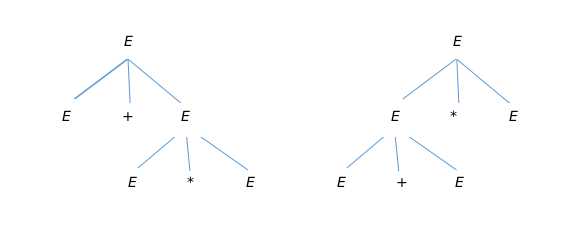
\includegraphics[scale=0.6]{ambiguita_due_alberi.png}
\centering
\end{figure}

\subsubsection{Eliminare le ambiguità da una grammatica}
In un mondo ideale sapremmo definire un algoritmo per eliminare le ambiguità dalle CFG per come le abbiamo definite. Purtoppo non esiste un modo per definire un algoritmo che data una qualsiasi CFG ci dice se essa è ambigua oppure no. Per fortuna nella pratica la situazione non è così drammatica. Per dirne una, nelle strutture sintattiche tipiche dei linguaggi di programmazione usuali esistono tecniche note per eliminare le ambiguità.
\\ \\
Utilizzeremo ancora l'esempio della sezione (1.4.1) per capire come è possibile eliminare l'ambiguità.
Possiamo notare che come prima cosa si hanno due cause di ambiguità:
\begin{enumerate}
	\item La precedenza degli operatori non è rispettata. Infatti, mentre nel primo caso applichiamo in "ordine" le derivazioni (prima $E+E$, poi alla seconda $E$ applichiamo $E*E$), nel secondo caso viene applicata prima $E*E$ e successivamente sulla \textit{prima} $E$ si applica $E+E$. Dovrebbe essere lecita solo la prima derivazione, quella "\textit{ordinata}".
	\item Una sequenza di operatori identici si può raggruppare sia da sinistra che da destra. Quindi, nal caso si ha $E+E+E$ ad esempio, visto che la somma (ma anche la moltiplicazione) sono associative, bisogna prendere una posizione e scegliere da che parte si decide di proseguire. La soluzione convenzionale è quella che prevede di raggruppare da sinistra.
\end{enumerate}


Il problema di imporre una precedenza si risolve introducendo alcune variabili, ognuna delle quali rappresenta le espressioni con lo stesso grado di "forza di legamento", secondo lo schema seguente:
\begin{enumerate}
	\item Un \textit{fattore} è un'espressione che non si può scomporre rispetto ad un operatore adiacente, * o +. Nel linguaggio delle espressioni i soli fattori sono i seguenti:
	\begin{enumerate}[(a)]
		\item Identificatori. Non è possibile separare le lettere di un identificatorie inserendo un operatore.
		\item Qualsiasi espressione fra parentesi, indipendentemente dal suo contenuto. Lo scopo delle parentesi è proprio quello di impedire che ciò che racchiudono diventi l'operando di un operatore esterno.
	\end{enumerate}
	\item Un\textit{termine} è un'espressione che non può essere scomposta dall'operatore +. Nell'esempio, in cui + e * sono i soli operatori, un termine è il prodotto di uno o più fattori. Per esempio il termine $a*b$ può essere scomposto se applichiamo l'associatività a sinistra e poniamo $a1 *$ alla sua sinistra. Infatti $a1*a*b$ può essere raggruppato come $(a1*a)*b$, che separa $a*b$. Se invece poniamo un termine additivo come $a1+ $ a sinistra o $+a1$ a destra, non possiamo spezzarlo. Il raggruppamento corretto di $a1+a*b$ è $a1+(a*b)$, mentre quello di $a*b+a1$ è $(a*b)+a1$.
	\item Per \textit{espressione} intenderemo d'ra in avanti qualsiasi espressione, comprese quelle che possono essere spezzate da un * o da un + adiacente. Nell'esempio, perciò, un'espressione è la somma di due o più termini. 
\end{enumerate}

\paragraph{Derivazioni a sinistra per esprimere ambiguità} Possiamo affermare che le derivazioni non sono necessariamente uniche, anche in grammatiche non ambigue. Ma in generale, in una grammatica non ambigua le derivazioni a sinistra (come quelle a destra) sono uniche.

\begin{ambiguitaSinistra}
Per ogni grammatica $G=(V,T,P,S)$ e per ogni stringa $w$ in $T^*$, $w$ ha due alberi distinti se e solo se ha due distinte derivazioni \textbf{a sinistra} da $S$.
\end{ambiguitaSinistra}

\paragraph{Dimostrazione} (Solo se) Esaminiamo la costruzione di una derivazione a sinistra a partire da un albero sintattico. Possiamo osservare che in corrispondenza di un nodo in cui gli alberi applicano produzioni diverse, anche le due derivazioni a sinistra applicano due produzioni diverse, e sono perciò distinte.
\\ \\
\subsubsection{Ambiguità inerente}
 Un linguaggio $L$ CFG si dice \textbf{inerentemente ambiguo} se tutte le sue grammatiche sono ambigue. Se anche solo una grammatica per $L$ non è ambigua, allora $L$ non è ambiguo. Anche se, per esempio, presa la stringa $a*a+a$ vista precedentemente, possiamo dire che esiste per essa una grammatica non ambigua.
 
 Infatti, la grammatica definita come
 \begin{enumerate}
 	\item $I \rightarrow a\medspace |\medspace b\medspace |\medspace Ia\medspace |\medspace Ib\medspace |\medspace I0\medspace |\medspace I1$
 	\item $F \rightarrow I\medspace |\medspace (E)$
 	\item $T \rightarrow F \medspace | \medspace T*F$
 	\item $E \rightarrow T\medspace |\medspace E+T$
\end{enumerate}
genera la stringa $a*a+a$ in modo non ambiguo con la seguente derivazione:

\begin{figure}[H]
\caption{Albero sintattico per $a+a*a$ da una grammatica non ambigua}
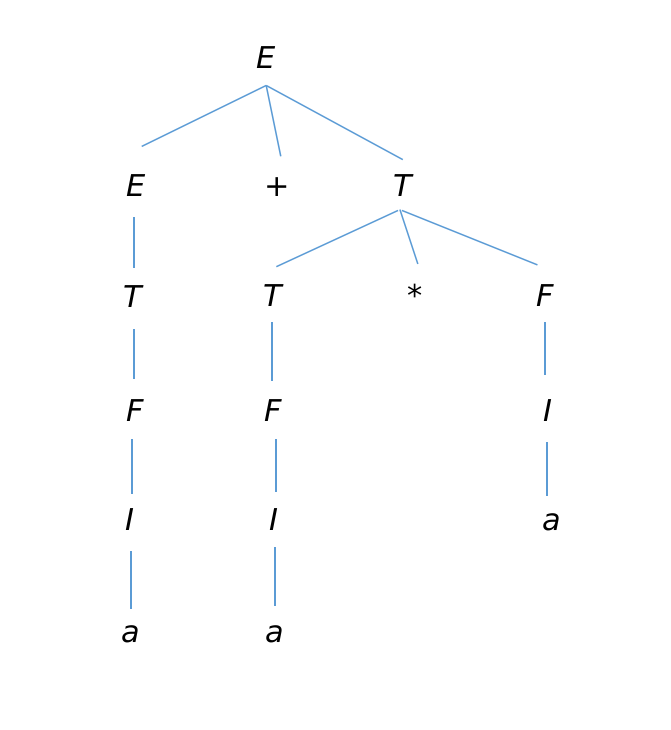
\includegraphics[scale=0.5]{albero_non_ambiguo_1.png}
\centering
\end{figure}  

\section{Alberi Sintattici}
Un albero sintattico è una rappresentazione grafica (ad albero) che mostra come una forma sentenziale o una stringa è stata ottenuta tramite le regole di derivazione.

\begin{alberoSintattico}
Data una CFG definita come $$G=(V,T,P,S)$$ l'albero sintattico è un albero tale che
\begin{enumerate}
	\item Ogni nodo interno è \textbf{etichettato} da una variabile;
	\item Ogni foglia è etichettata da una variabile, oppure un simbolo terminale o ancora da $\varepsilon$. Se è etichettata con $\varepsilon$ allora è l'unico figlio riscontrato.
	\item Se un nodo è etichettato con A (variabile) e i rispettivi figli sono etichettati da sinistra verso destra con $X_1,X_2,X_3,...,X_k$, allora $A \rightarrow X_1,X_2,X_3,...,X_k \in P$ (ovvero A è una produzione della grammatica).
\end{enumerate}
\end{alberoSintattico}

Un esempio pratico di albero sintattico: data la CFG definita come
\begin{equation}
E \rightarrow I\medspace |\medspace E+ E\medspace |\medspace E*E\medspace |\medspace (E)\medspace \medspace e \medspace \medspace I \rightarrow a\medspace |\medspace b \medspace |\medspace Ia\medspace |\medspace I0\medspace |\medspace I1
\end{equation}


\begin{center}
%%creazione dell'albero secondo la CFG data
\begin{tikzpicture}[->,>=stealth',level/.style={sibling distance = 2cm/#1,
  level distance = 1.5cm}] 
\node [arn_n] {E}
    child{ node [arn_n] {E} 
            child{ node [arn_r] {I}}            
    }
    child{ node [arn_r] {+}
  	}
  	child{	node[arn_r] {E}
  	}
; 
\end{tikzpicture}
\end{center}
abbiamo che l'albero sintattico ottenuto è un albero \textbf{radicato} e \textbf{ordinato}. Si può notare che i \color{blue}nodi interni \color{black} rappresentano i passaggi per arrivare alle \color{red}foglie\color{black}. Difatti è possibile ricostruire il processo di derivazione: $$E \rightarrow E \medspace + \medspace E \rightarrow I \medspace + \medspace E$$

\subsubsection{Inferenza, derivazioni e alberi sintattici}
Ognuna delle nozioni viste fino ad ora  per descrivere una grammatica dà essenzialmente gli stessi risultati sulle stringhe. Quindi possiamo dire che vale il seguente teorema
\begin{eqEnunciati}
data una grammatica $G=(V,T,P,S)$, i seguenti enunciati si equivalgono.
\begin{enumerate}
	\item l'inferenza ricorsiva stabilisce che la stringa $w$ è nel linguaggio della variabile A.
	\item $A\Rightarrow^{*} w$.
	\item $A\Rightarrow^{*}_{lm} w$.
	\item $A\Rightarrow^{*}_{rm} w$.
	\item esiste un albero sintattico con radice A e prodotto $w$.
\end{enumerate}
\end{eqEnunciati}
Se escludiamo l'inferenza ricorsciva, definita solo per stringhe terminali, le altre condizioni -l'esistenza di derivazioni generiche, destre o sinistre, e di alberi sintattici - sono equivalenti anche se $w$ contiene variabili.
\begin{figure}[H]
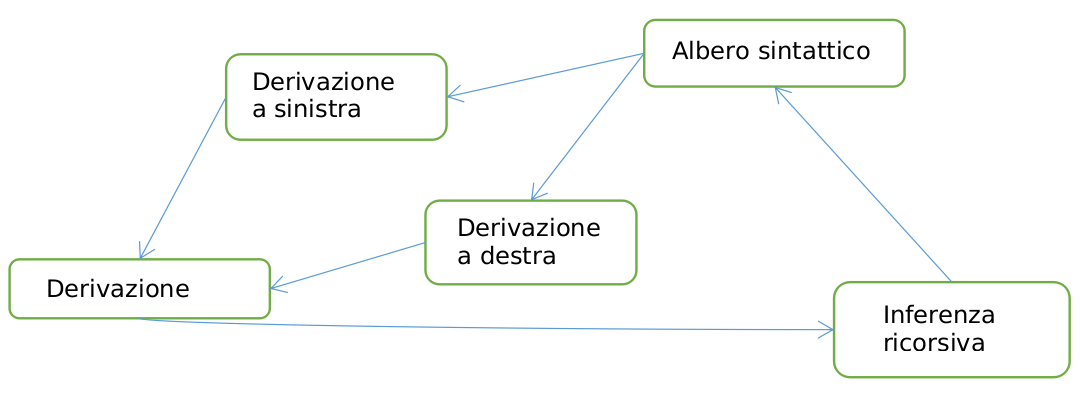
\includegraphics[scale=0.4]{derivazione_inf_albero.png}
\centering
\end{figure}

Banalmente, se $w$ ha un derivazione a sinistra (o a destra) da A, allora avrà una anche una \textit{derivazione}, dato che una derivazione a sinistra (o a destra) è una derivazione.
\\\\
\subsubsection*{Dalle inferenze agli alberi}
\paragraph*{\textbf{Teorema}} Sia $G=(V,T,P,S)$ una CFG. Se la procedura di inferenza ricorsiva indica che la stringa terminale $w$ è nel linguaggio della variabile A, allora esiste un albero sintattico con radice A e prodotto $w$.
\paragraph*{DIMOSTRAZIONE} La dimostrazione è un'induzione sul numero di passi usati per dedurre che $w$ è nel linguaggio di A.

\subparagraph*{BASE} Un solo passo. In questo caso deve essere stata usata solo la base della procedura di inferenza. Di conseguenza deve esistere per forza una produzione $A \rightarrow w$. L'albero sotto riportato, in cui esiste una sola foglia per ogni posizione di $w$, soddisfa le condizioni degli alberi sintattici per la grammatica G, e ha evidentemente prodotto $w$ e radice A.

\begin{figure}[H]
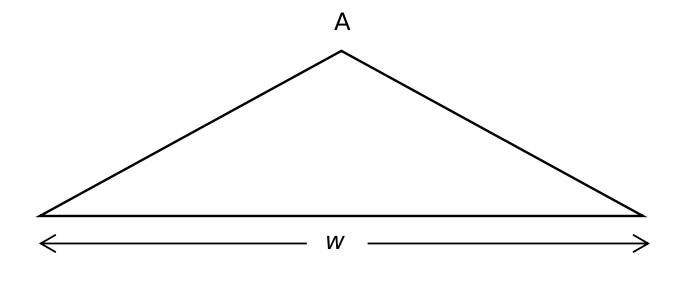
\includegraphics[scale=0.4]{albero_A_w.png}
\centering
\end{figure}

\subparagraph*{INDUZIONE} Supponiamo di aver dedotto che $w$ è nel linguaggio di A dopo $n+1$ passi di inferenza, e che l'enunciato del teorema sia valido per tutte le stringhe $x$ e variabili $B$ tali che l'appertenenza di $x$ al linguaggio $B$ si deduca in $n$, o meno, passi di inferenza. Questa inferenza impiega una certa produzione per A, poniamo $A \rightarrow X_1, X_2,...,X_k$, dove ogni $X_i$ è una variabile oppure un terminale.
\\ \\
Possiamo scomporre $w$ in $w_1,w_2,...,w_k$ soddisfacendo le seguenti clausole:
\begin{enumerate}
	\item Se $X_i$ è un terminale, allora $w_i = X_i$, cioè $w_i$ consiste solamente di questo terminale.
	\item Se $X_i$ è una variabile, allora $w_i$ è una stringa di cui è stata precedentemente dedotta l'appartenenza al linguaggio di $X_i$. In altre parole l'inferenza relativa a $w_i$ ha richiesto al massimo $n$ degli $n+1$ passi dell'inferenza per la quale $w$ si trova nel linguaggio di A. Non richiede tutti gli $n+1$ passi perchè il passo finale, che si avvale della produzione $A \rightarrow X_1, X_2, ..., X_k$, non è sicuramente parte dell'inferenza di $w_i$. Di conseguenza possiamo applicare l'ipotesi induttiva a $w_i$ e $X_i$, e concludere che esiste un albero sintattico con prodotto $w_i$ e radice $X_i$.	
\end{enumerate}

\begin{figure}[H]
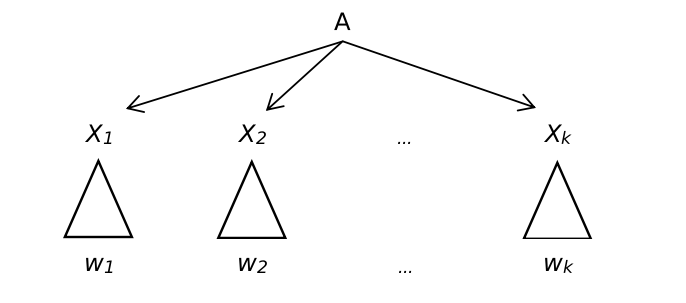
\includegraphics[scale=0.5]{derivazione_inf_albero_mult.png}
\centering
\end{figure}

Construiamo poi un albero come quello soprastante.

Il nodo di ciascuna $X_i$ diventa la radice di un sottoalbero con prodotto $w_i$. Nel caso in cui $X_i$ sia un simbolo terminale, questo sottoalbero è un albero banale con un solo nodo etichettato con $X_i$. Nel caso in cui $X_i$ è una variabile, invochiamo l'ipotesi induttiva per sostenere che esiste un albero con radice  $X_i$ e prodotto $w_i$. 

L'albero costruito in questo modo ha radice A e prodotto formato dai prodotti dei sottoalberi, concatenati da sinistra a destra. la stringa è $w_1, w_2, ... ,w_k$ ovvero $w$. 

\end{document}
